
%%% Local Variables:
%%% mode: latex
%%% TeX-master: "../../doktorarbeit"
%%% End:
\chapter{The effects of rotation}
In this chapter we study the effects rotation have on the GW signal. 
We present three models based on the same progenitor, two rotating models and one non-rotating.
This allows us to study how the signal GW is effected by rotation. 


\section{Supernova Models}
We present the GW signal from three models based on the progenitor of
\cite{heger_05}, which is a solar-metallicity star with a ZAMS mass of $15 \msun$.
The progenitor was developed, taking into account the effects of magnetic fields and rotation,
from ZAMS to the onset of iron-core collapse. The inclusion of magnetic fields lead to an overall
reduction of the final rotation rate of the iron core, compared to a star evolved without magnetic
fields. The main difference between the three models is their rotation profiles. One of the models
uses the profile of the progenitor (m15r), an other has a enhanced rotation profile (m15fr),
in the last model the rotation rate has been set to zero throughout the star (m15nr)
In \fig{figp2:rot} we show the rotation profiles of m15fr and m15fr.
\begin{itemize}
\item \textbf{m15fr:} The rotation profile of model m15fr has, by hand, been set to a constant rotation rate of 0.5 rad/s
throughout the inner core of the star. At a radius of 1731 km the rotation profile changes
to a linearly decaying profile (\fig{figp2:rot}). The model was simulated using the Yin-Yang grid, the 
two grid patches had an initial resolution of 400 cells, 56 cells and 144 cells in the radial, polar and
azimuthal directions, respectively. This corresponds to a 2 degree angular resolution. 
After the initial shock expansion halts around $60$ ms post bounce the average shock radius decreases slightly.
Between $\sim 80 - 160$ ms post bounce the shock front is on average more or less stationary. 
The shock starts to expand roughly $160$ ms after core bounce and soon after shock revival sets in.
The average shock reaches $2000$ km around $\sim 330$ ms after core bounce.
In the time before shock revival, the post-shock flow is dominated by a strong spiral SASI mode. The SASI sets in around
$\sim 100$ ms post bounce.
\item \textbf{m15r:} The initial rotation profile of model m15r is exactly that of the progenitor \citep{heger_05}, without
any artificial changes made by hand. The rotation profile as a function of radius can be seen in \fig{figp2:rot}.  
The model was simulated using the Yin-Yang grid, the two grid patches had an initial resolution of 400 cells, 
56 cells and 144 cells in the radial, polar and azimuthal directions, respectively. This corresponds to a 2 degree angular resolution.
For the first $\sim 80$ ms after bounce, the evolution of the average shock radius of model m15r closely resembles the
one seen in model m15fr. However, around $100$ ms the average shock radius starts to decrease. Unlike model m15fr, strong 
SASI activity does not develop in model m15r, the flow in the post-shock region is instead dominated by hot-bubble convection. There
is, however, some low amplitude dipole deformation of the shock front (see \fig{figgp2:sasi}).
The average shock radius continue until
$\sim 200$ ms post bounce when the Si-O shell interface falls through the shock. The decrease density in front of the shock leads
to decreased ram pressure and a transient period of shock expansion. At $\sim 240$ ms post bounce the expansion subsides and
the shock front once more begins to retreat, a trend which continues until the end of the simulation.  
\item \textbf{m15nr:} In model m15nr the initial rotation rate was set to zero at all radii. The model was simulated using the Yin-Yang grid, the
two grid patches had an initial resolution of 400 cells, 28 cells and 72 cells in the radial, polar and
azimuthal directions, respectively. Which means that model m15nr was simulated with an angular resolution that is
two times coarser than the other two models (4 degrees). Initially the shock expands and reaches a local maximum around $60$ ms after bounce,
from this point the shock radius steadily decreases until the Si-O shell interface falls through the shock. The decreased accretion rate
leads to a transient period of shock expansion, until the shock eventually starts to recede once more. Except for the fact that
the average shock radius is generally larger in model m15nr, model m15nr is similar to model m15r in terms of the evolution of the average shock
radius. However, unlike model m15r, model m15nr develops strong SASI activity. In this model the SASI activity is dominated by the sloshing mode.
The mode develops around $\sim 120$ ms after core bounce and peaks around $\sim 230$ ms post bounce. After the peak in activity 
the SASI mode gradually decays towards the end of the simulation.   
\end{itemize}
\begin{figure}[ht]           
\centering                            
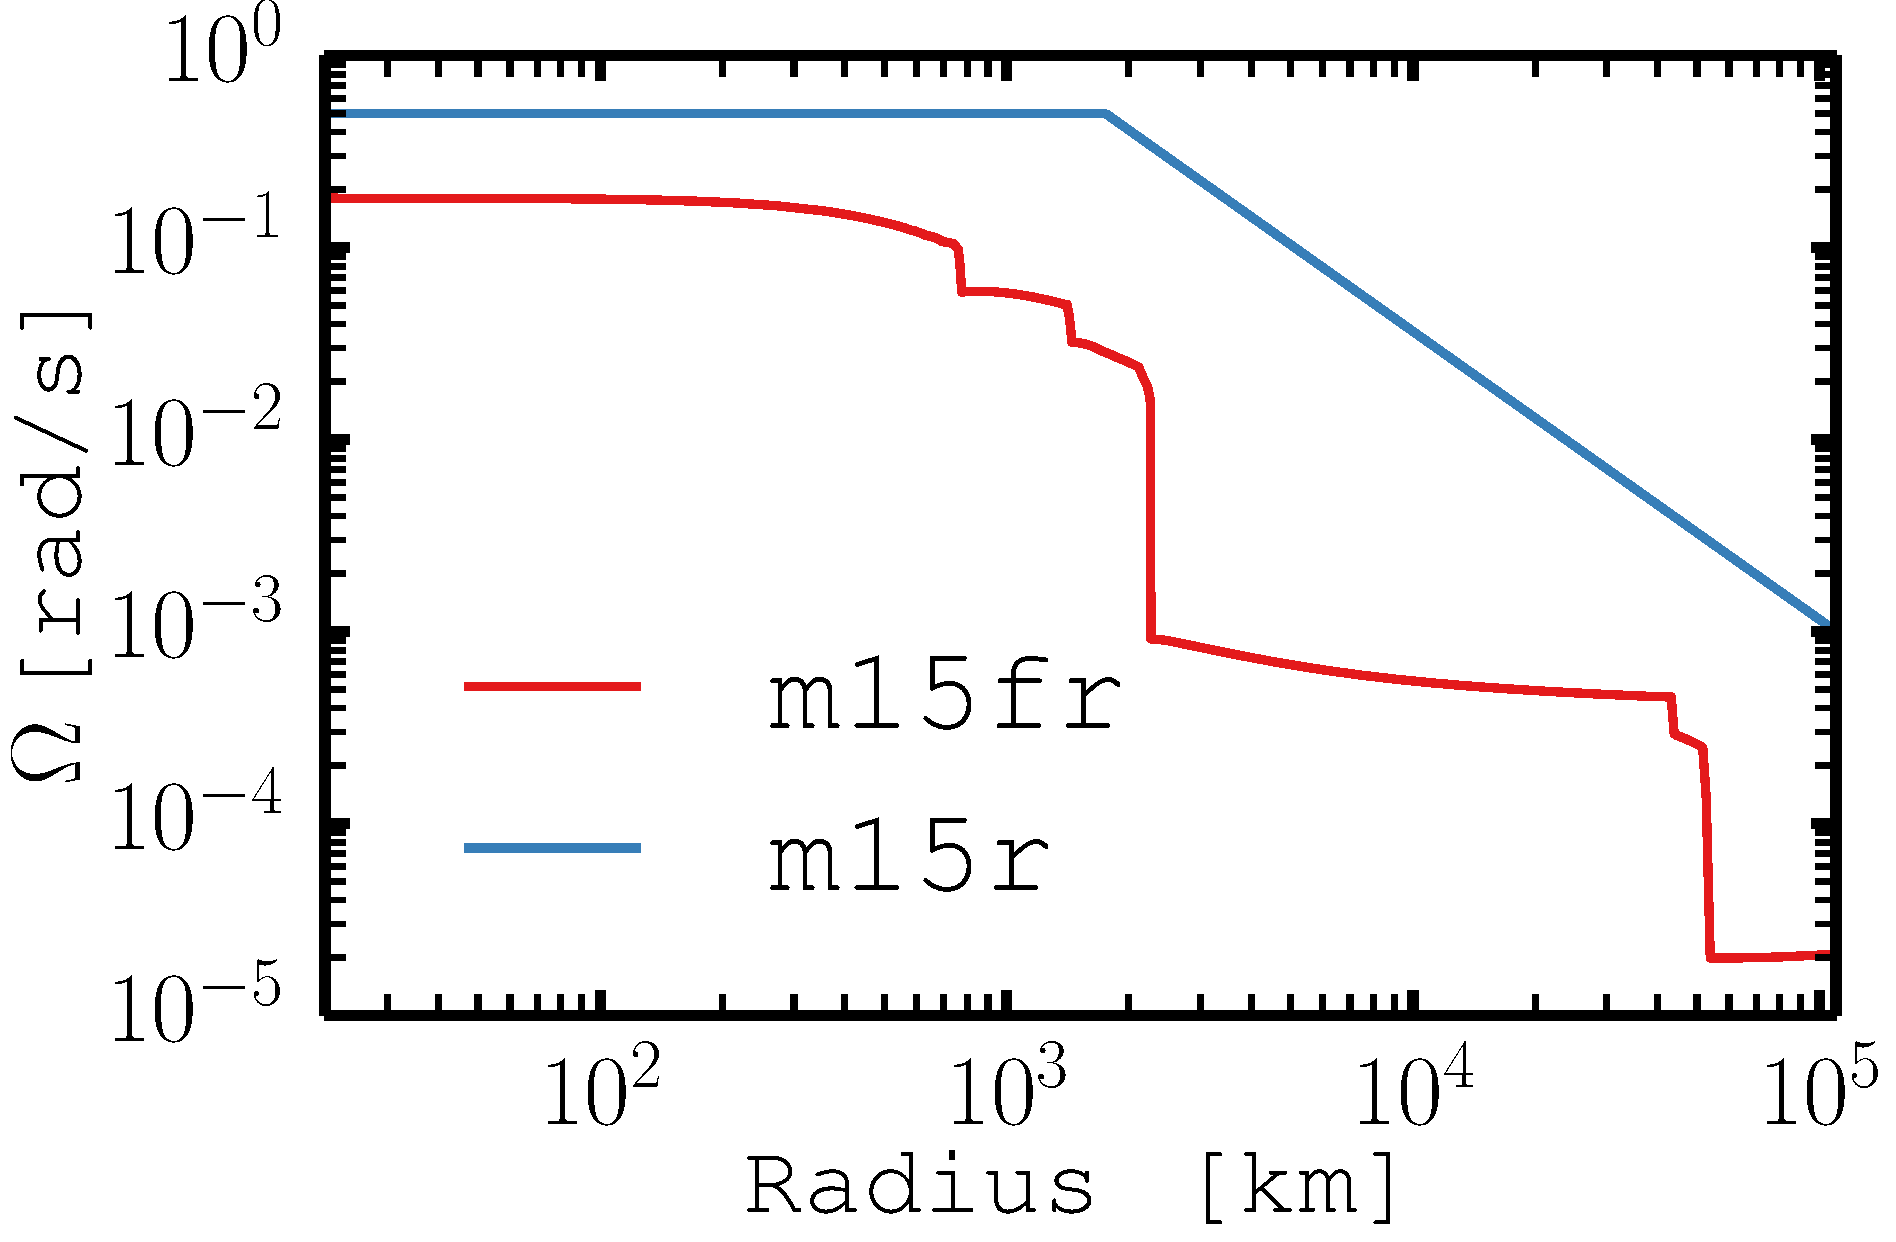
\includegraphics[width=0.99\textwidth]{./images/paper2/rot.pdf}
\caption{The radial rotation profiles for the two rotating models. The red line represents model 
m15fr and the blue line represents m15r. \label{figp2:rot}}
\end{figure}
\begin{figure}[ht]         
\centering                            
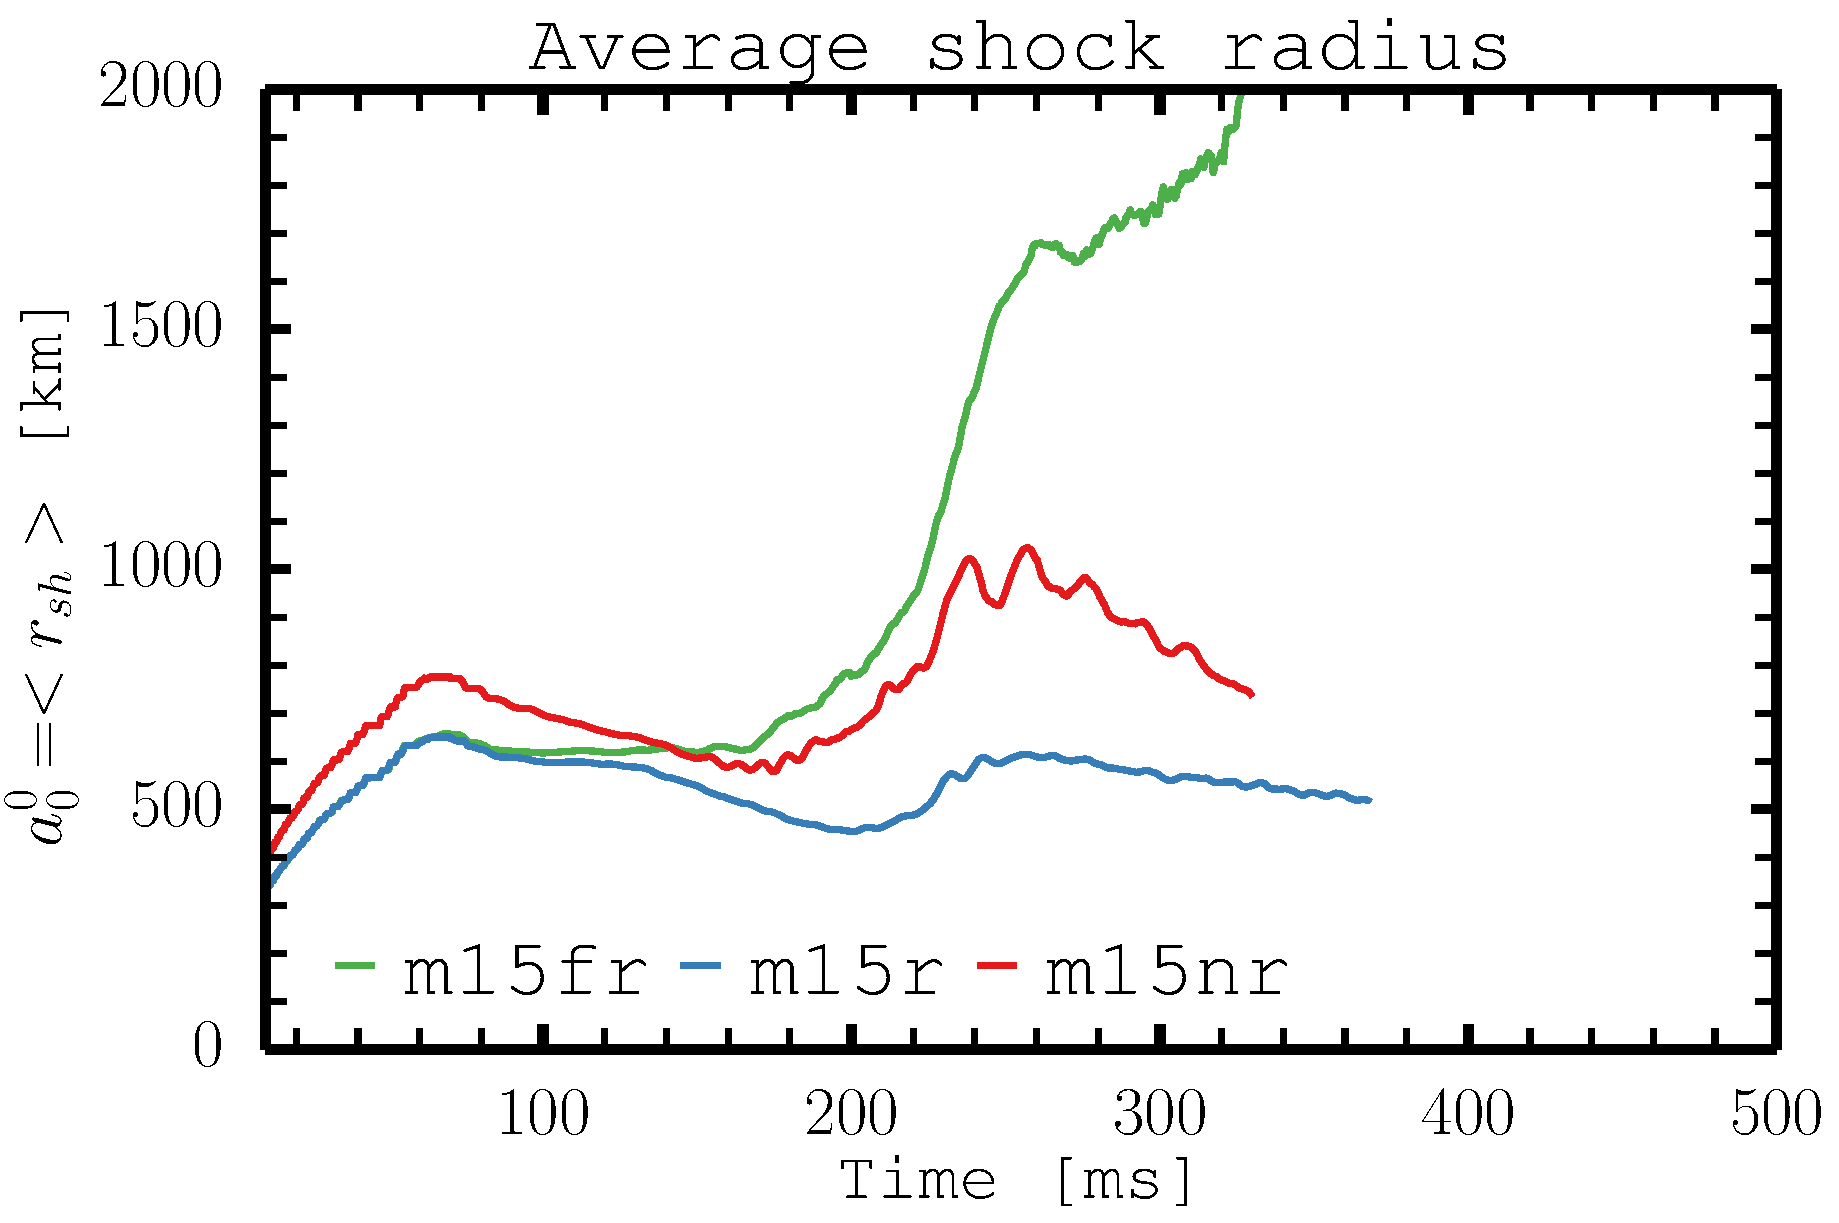
\includegraphics[width=0.99\textwidth]{./images/paper2/rsh.pdf}
\caption{Average shock radius for model m15fr (green), m15r (blue), and m15nr (red) as a function of 
time after core bounce. The average shock radius is defined as the $(l,m) = (0,0)$ expansion coefficient of the shock surface into 
spherical harmonics (\eq{eq:alsph}). \label{figp2:rsh}}
\end{figure}
\begin{figure}[ht]         
\centering                            
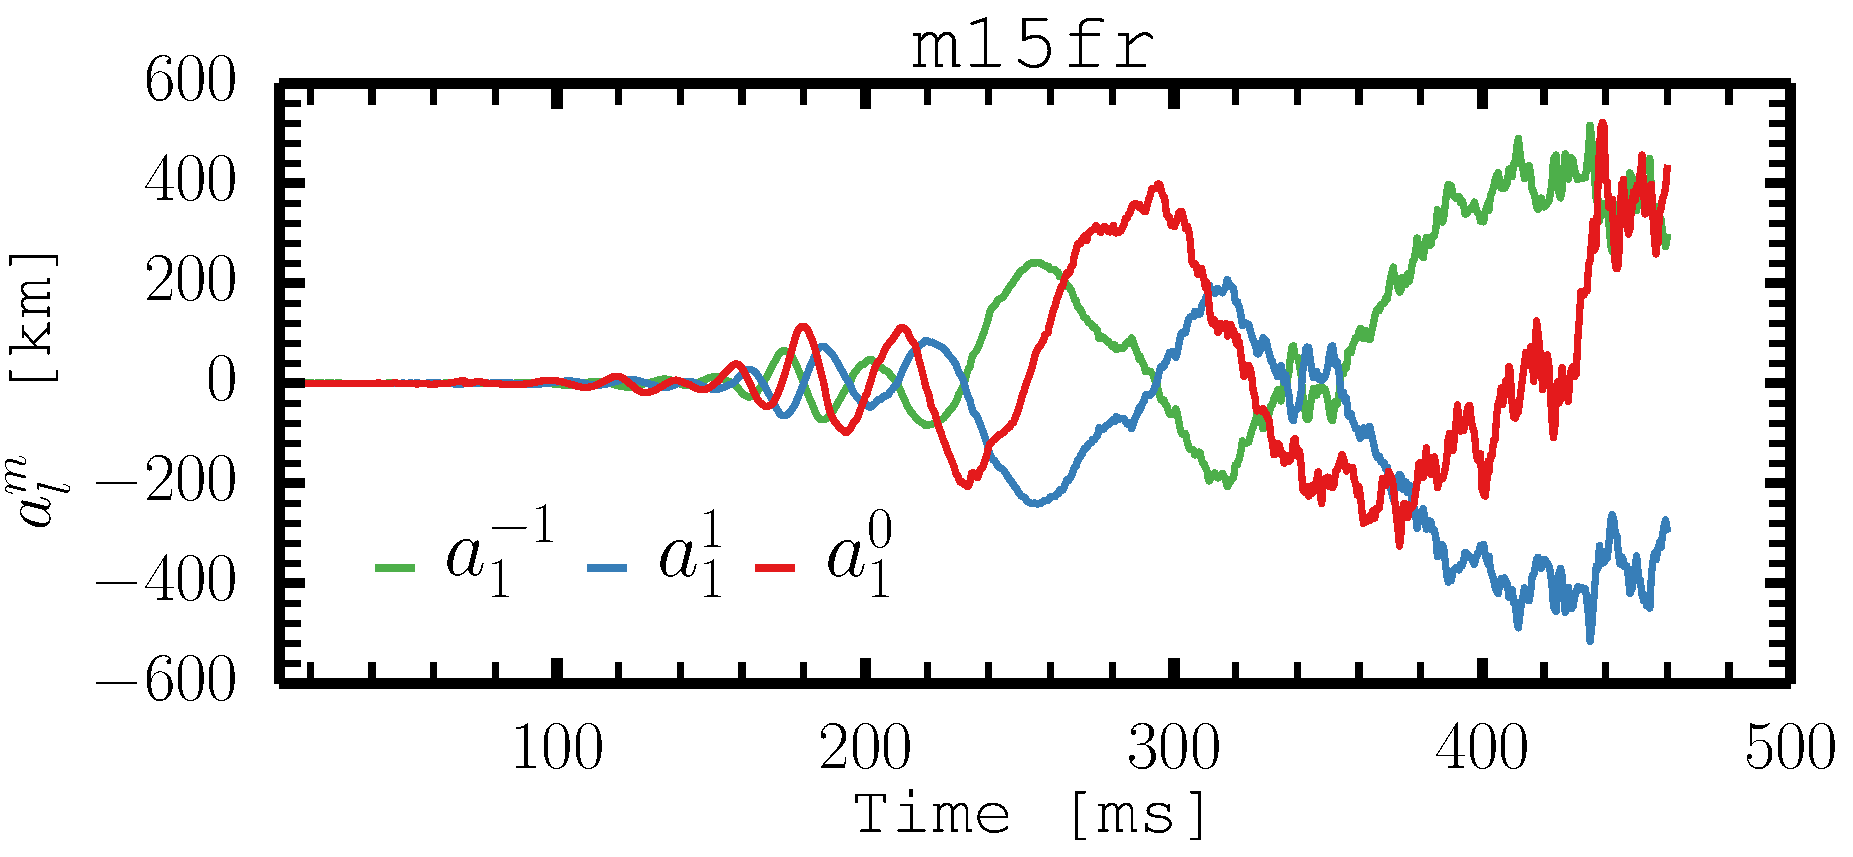
\includegraphics[width=0.9\textwidth]{./images/paper2/sasi_fr.pdf}
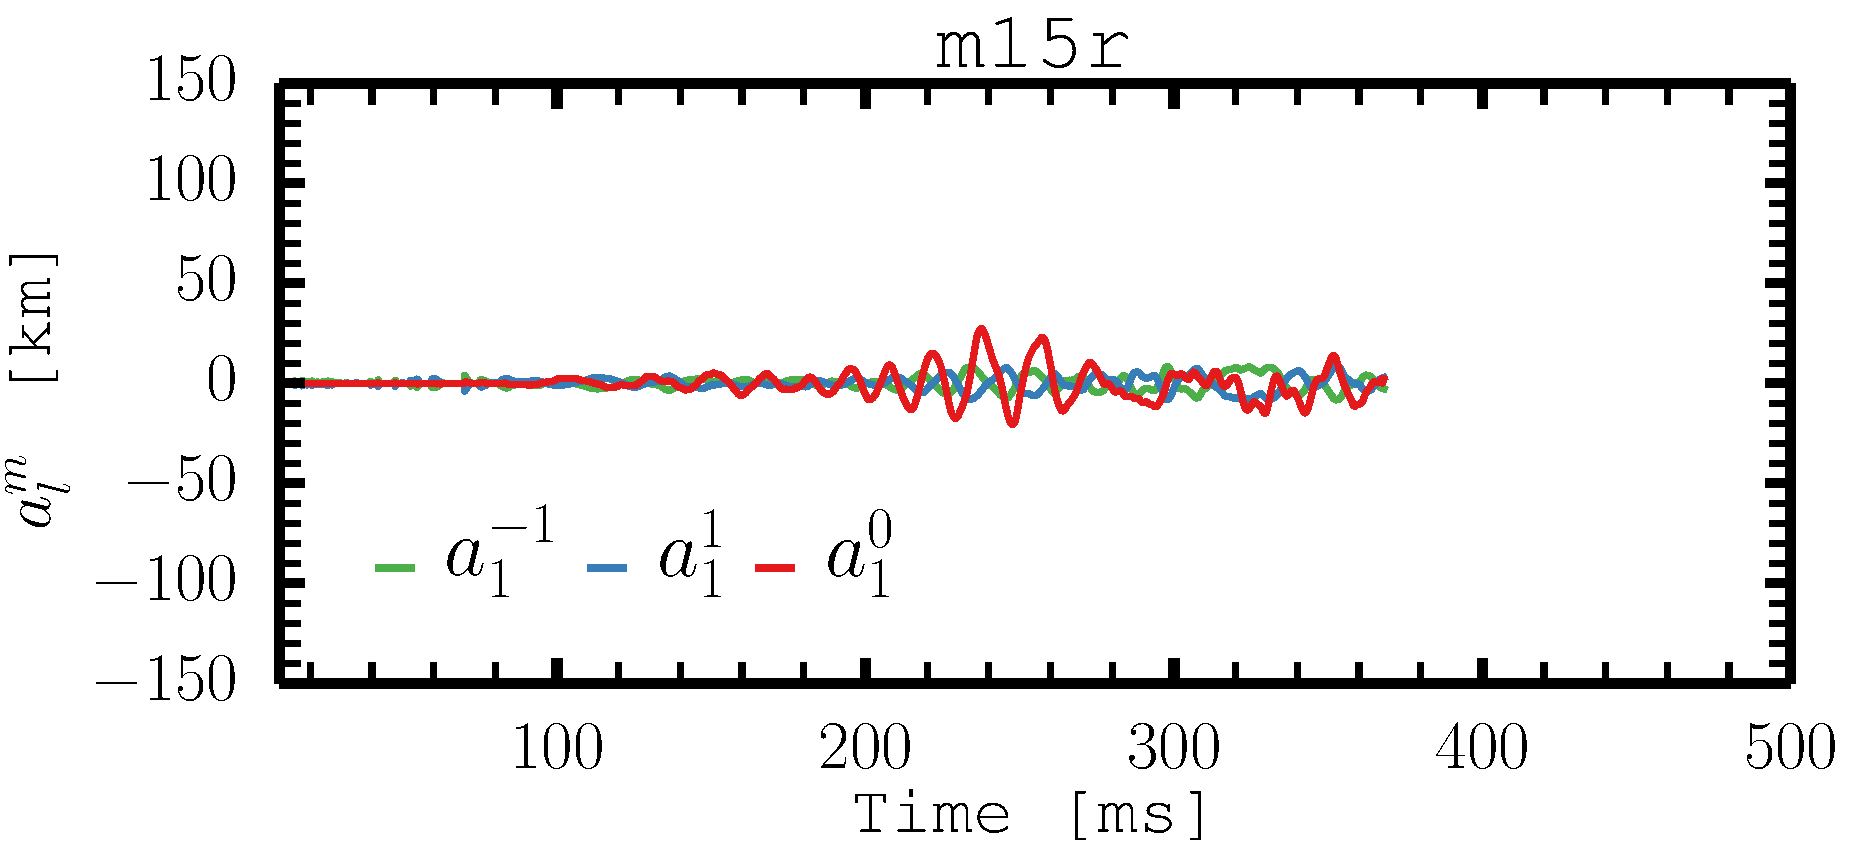
\includegraphics[width=0.9\textwidth]{./images/paper2/sasi_r.pdf}
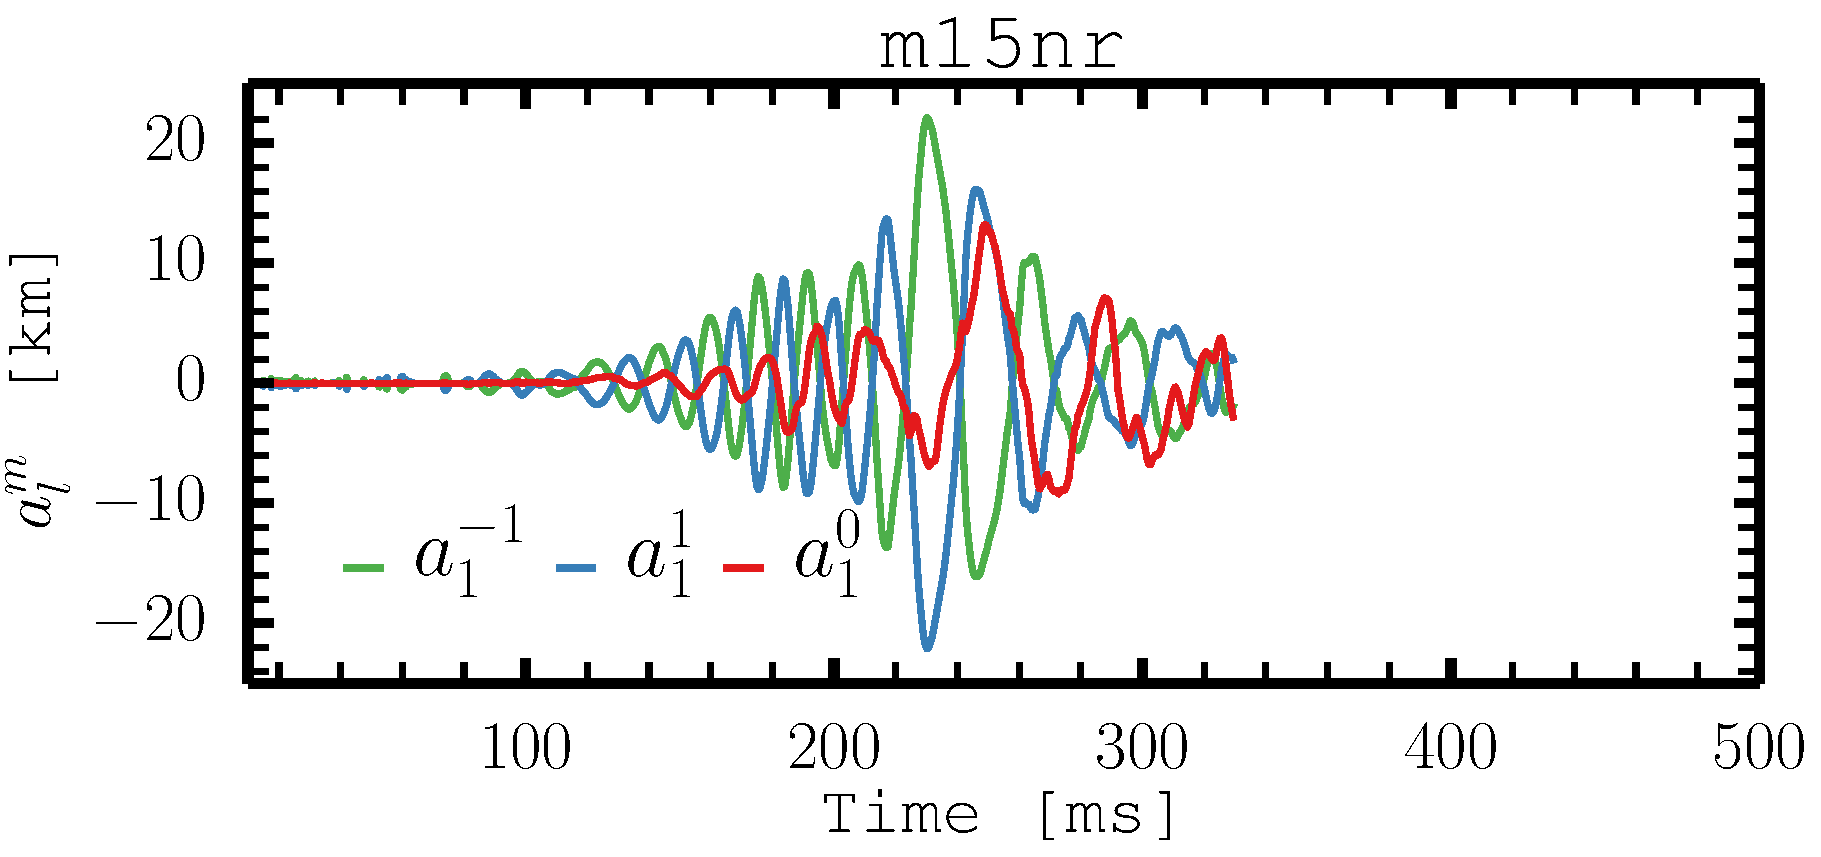
\includegraphics[width=0.9\textwidth]{./images/paper2/sasi_nr.pdf}
\caption{The $(l,m) = (1,0)$, $(1,1)$, and $(1,-1)$ coefficients of the decomposition of the shock surface into spherical harmonics
as a function of time after bounce, see \eq{eq:alsph}. From the top to bottom: Model m15fr, model m15r, and model m15nr. \label{figp2:sasi}}
\end{figure}

\section{Results}
\subsection{Qualitative description of the gravitational wave signals}
The GW signals from the rotating models do not qualitatively differ significantly from
the signals presented in chapter~\ref{ch:firstpaper}. In \fig{figp2:amps} we show the
GW amplitudes generated by asymmetric mass motions for models m15fr, m15r and m15nr.
The two columns shows the amplitudes for two different observer orientations,
the right and left Colon represent observers situated along the x-axis (equator) and z-axis (pole) of the Yin grid-patch,
respectively. The rows are order by progenitor, in order of decreasing initial rotation, and from the top
shows m15fr, m1fr and m15nr. Vertical lines indicates episodes of strong SASI activity.
The corresponding amplitude spectrograms (see \eq{eqSA:STFT}) for a sliding window of $50 \, \mathrm{ms}$ are shown 
in Fig.~\ref{fig:totspec}. The spectrograms show the sum of the squared Fourier
components of the cross and plus polarisation modes,
$\text{STFT}[{A_+}]^2 + \text{STFT}[{A_{\times}}]^2$. Before applying the
DFT we convolve the signal with a Kaiser window with shape parameter $\beta = 2.5$. Frequencies
below $50 \, \mathrm{Hz}$ and above $1100  \, \mathrm{Hz}$ are filtered out of the resulting spectrograms. 

In all three models, an initial phase of quiescence is followed by a phase of rather stochastic emission, 
during with the typical amplitudes are on the order of a few cm. Model m15fr have the largest amplitude, of the three
models, but at the same time the non-rotating model (m15nr) show larger amplitudes than the moderately rotating model (m15r).
There seems to be no clear correlation between the strength initial rotation rate and the strength of the GW emission. 
The spectrograms (\fig{figp2:spec)} show the familiar low-frequency and a high-frequency components that we saw in the
four models presented in chapter~\ref{ch:firstpaper}.

During the SASI phase of m15fr, we see a low-frequency signal component in addition 
to the high-frequency stochastic component. Both strong low-frequency and high-frequency
emission is visible in the upper row of \fig{figp2:spec}. Both signal components
are broader in model m15fr than in the other two models, to the point where the two components almost
overlap. After the shock starts to expand the overall GW amplitudes are somewhat reduced, but
both low-frequency and high-frequency emission continues until the end of the simulation.

Of the three models, model m15r produces the weakest GW signal. The GW amplitudes
never exceeds $1.5$ cm, for both observer directions. Furthermore, the signal is strongly reduced in the
time period between $180$ and $250$ ms post bounce. During this time high-frequency emission
completely subsides and only very weak low-frequency emission is present in the signal.
Around $\sim 250$ ms post bounce high-frequency emission sets in once more, 
at the same time the low-frequency emission ceases. 

The non-rotating model (m15nr) is characterised by a relatively long initial quiescent phase, compared to the two
rotating models. Low amplitude low-frequency GW emission set in around $\sim 125$ ms after bounce. The low-frequency
signal component increases in strength until reaching a maximum around $175$ ms after core bounce.
Approximately $25$ ms after the onset of low-frequency emission, high-frequency emission develops around
$\sim 150$ ms after core bounce. After they developed, the two signal components persists, varying in
strength, until the end of the simulation.

\begin{figure}           
\centering                            
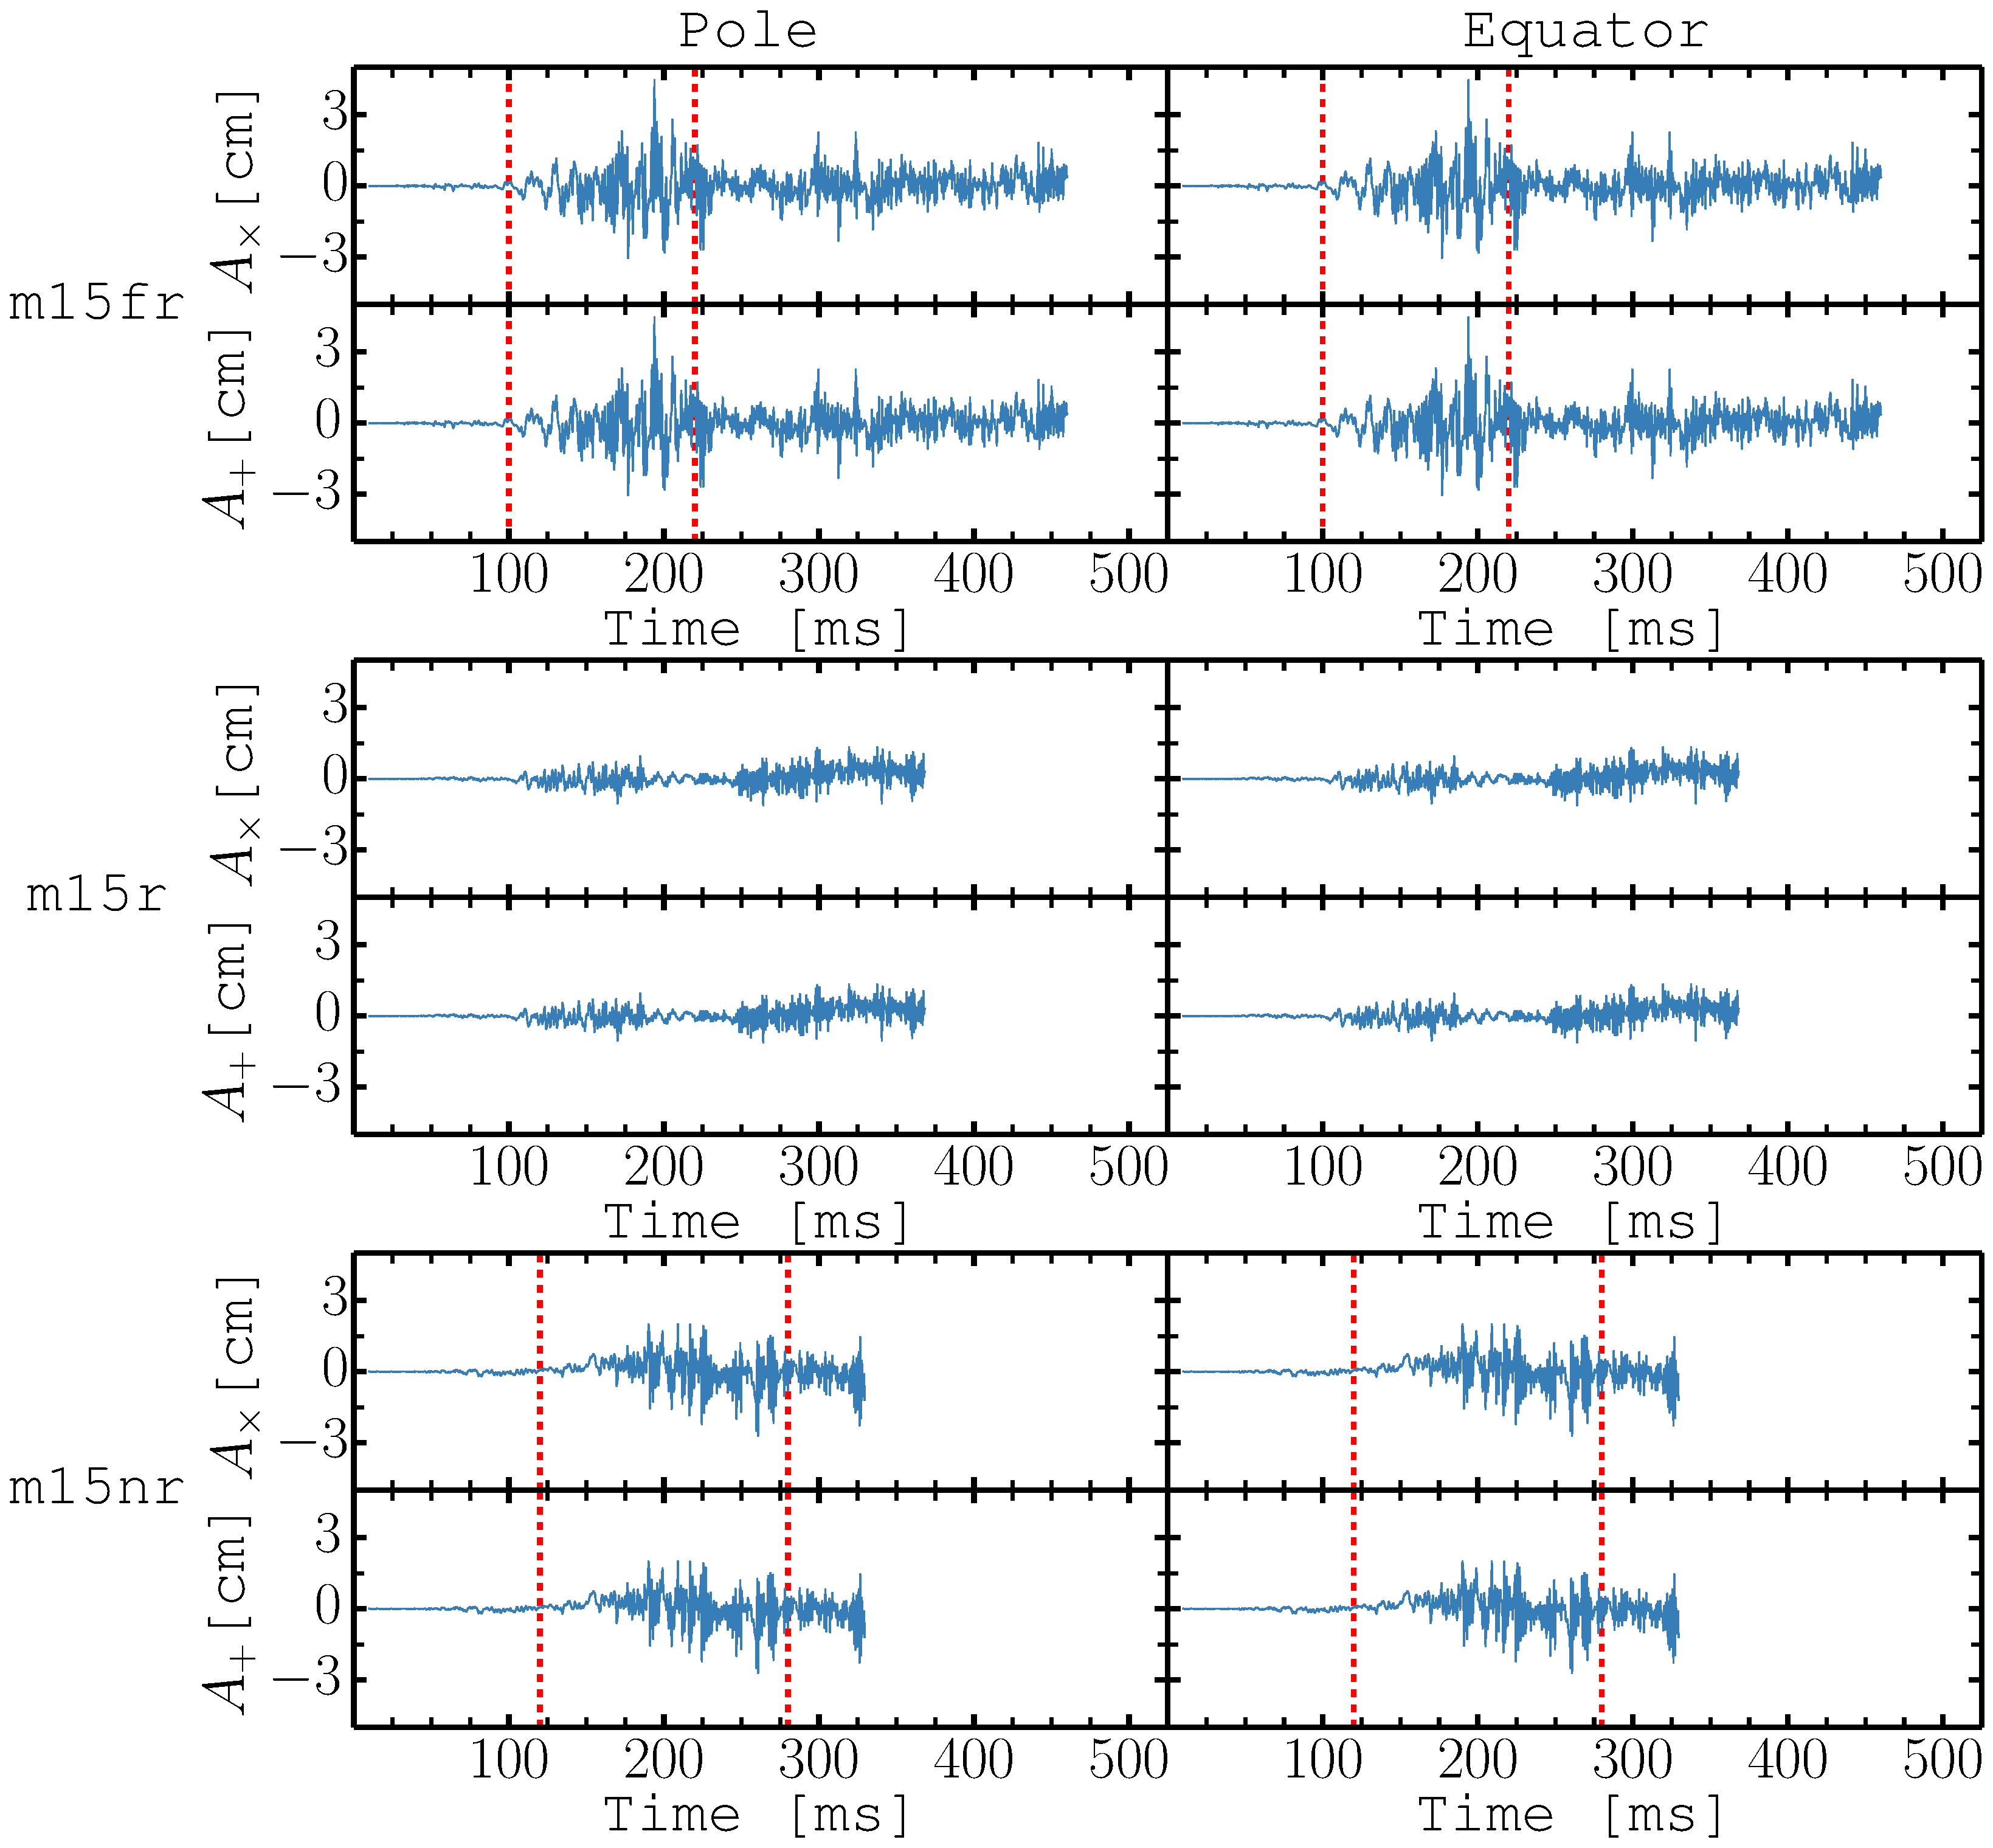
\includegraphics[width=0.99\textwidth]{./images/paper2/amps.pdf}
\caption{GW amplitudes $A_+$ and $A_\times$ as functions of time after core bounce.
  From the top: m15fr, m15r, and m15nr, respectively. 
  The two columns show the amplitudes for two different viewing angles: an observer
  situated along the $z$-axis (pole; left) and an other observer along the $x$-axis (equator; right) of the Yin grid patch, respectively.
  Episodes of strong SASI activity occur between the vertical red lines.  \label{figp2:amps}}
\end{figure}
\begin{figure}[ht]
\centering                            
\includegraphics[width=0.99\textwidth]{./images/paper2/rotspec.pdf}
\caption{Amplitude spectrograms for a sliding window of 50 ms and two different observer
  directions, summed over the two polarisation modes 
  ($|\widetilde{A}_+|^2 + |\widetilde{A}_\times|^2$). The
  different rows show the results for models m15fr, m1fr, and m15nr. (top to bottom).
  The two columns shows the spectrograms for two different viewing angles, the right and left column represent
  observers situated along the z-axis (pole) and x-axis (equator) of the Yin grid, respectively.
  The time is given in ms after core bounce. Vertical lines bracket SASI episodes. All panels have been normalised by the same global factor.
  The colour bar is given in a logarithmic scale. \label{figp2:spec}}
\end{figure}

\section{Excitation of gravitational waves}
In chapter~\ref{ch:firstpaper} we studied the hydrodynamical instabilities responsible for GW emission in detail.
We found that GWs are mainly excited in four ways. SASI activity leads to low-frequency by inducing an asymmetric mass distribution in the post-shock and by exciting forced non-resonant g-modes in the PNS. 
The forced g-modes are excited due to the  SASI modulated accretion flow onto the PNS 
and their frequency is set by the SASI frequency. High-frequency emission is caused by the propagation of
resonant g-modes in the PNS surface layer, the typical frequency of these oscillations is given by the
Brunt-V\"{a}is\"{a}l\"{a}-frequency in the PNS surface layer. Resonant g-modes are excited in two ways.
Firstly, by downdrafts from the post-shock layer impinge the PNS surface. Strong downflows can be created by SASI activity and overturn of convective plumes. Resonant g-modes are also excited, in the PNS surface layer,
as plumes from the unstable layer beneath overshoot into the surface layer.
For the four models presented in chapter~\ref{ch:firstpaper}, we found that PNS convection was the main diver
of this process and that downflows, while downflows from the post-shock layer provided a secondary and smaller
contribution (with model dependent variations in relative importance of the two).

These conclusions hold true for the three models presented in this chapter as well, with one notable
exception. In the two rotating models, model m15fr and model m15r, the GW signal generated by PNS convection 
is significantly reduced. When rotation is added to the simulations the PNS initially develops a positive
angular momentum gradient in the PNS convection layer, which acts as a stabiliser and weakens PNS
convection \citep{janka_01b}. 
The basic physical picture is that, when a buoyant plume propagates outwards its rotation rate
is less than that of the surrounding medium and it, consequently, experiences a weaker centrifugal force.
The effect of rotation is, therefore, to exact a force acting against the outwards propagation of the plume.
Angular momentum transfer by convection will eventually flatten the rotation profile within the PNS and 
the stabilising effect provided by rotation will gradually decrease with time.

Based solely on the stabilising effects rotation have on PNS convection we would expect an overall 
reduction of high-frequency GW emission in the two rotating models. However, the picture is not
so simple. We have to consider how well the Brunt-V\"{a}is\"{a}l\"{a}-frequency in the PNS surface overlaps with
the typical SASI and convective timescales. The compactness of the PNS tends to increase with
progenitor mass, which results in a higher Brunt-V\"{a}is\"{a}l\"{a}-frequency \citep{mueller_13}.
SASI activity and neutrino driven convection in the post-shock layer operates at relative long time-scales.
Consequently, the spectrum of the forcing and the natural g-mode frequency will overlap better
in model based on a low mass progenitor, with a less compact PNS, than a more massive model. 
This is in fact reflected in the four models we study in chapter~\ref{ch:firstpaper},
the contribution to the high-frequency emission by convective plumes striking the PNS from above
is relative high in model s11.2 (see \fig{fig:cuts}).
We also have to consider the effects of the spiral SASI mode.
The strong influence exerted by the spiral mode on the PNS, through a coherent large scale
modulation of the accretion flow onto the PNS, not only effectively perturbs the surface, 
but can also reaches into the interior of the PNS and influence the convective layer.


\begin{figure}[ht]         
\centering                            
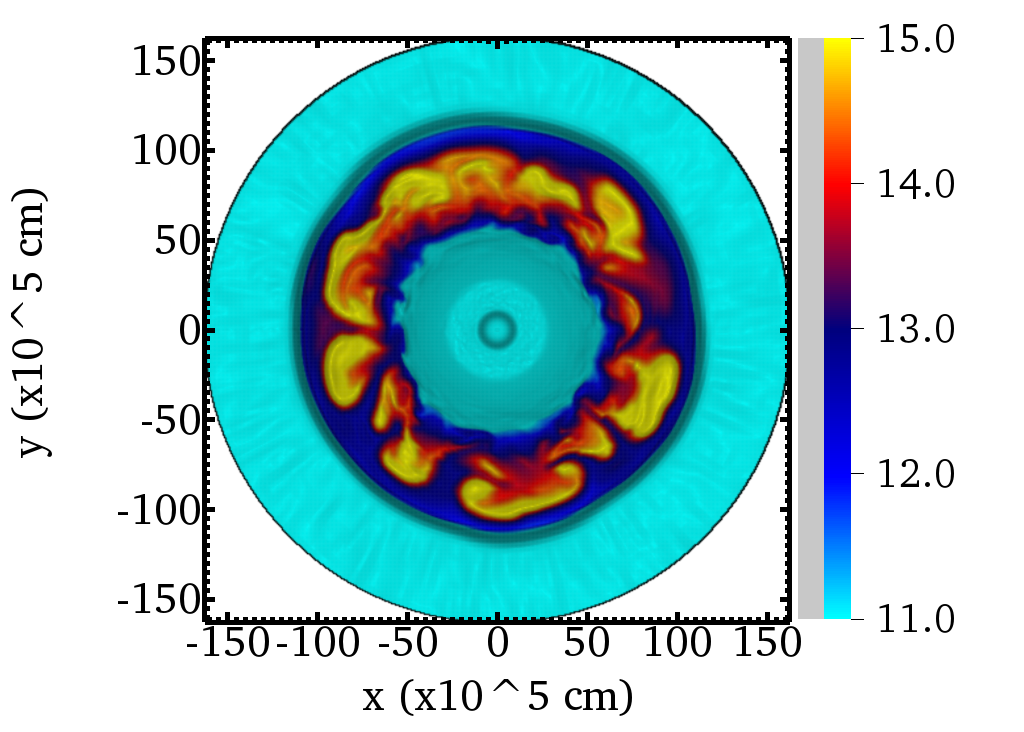
\includegraphics[width=0.49\textwidth]{./images/paper2/1.png}
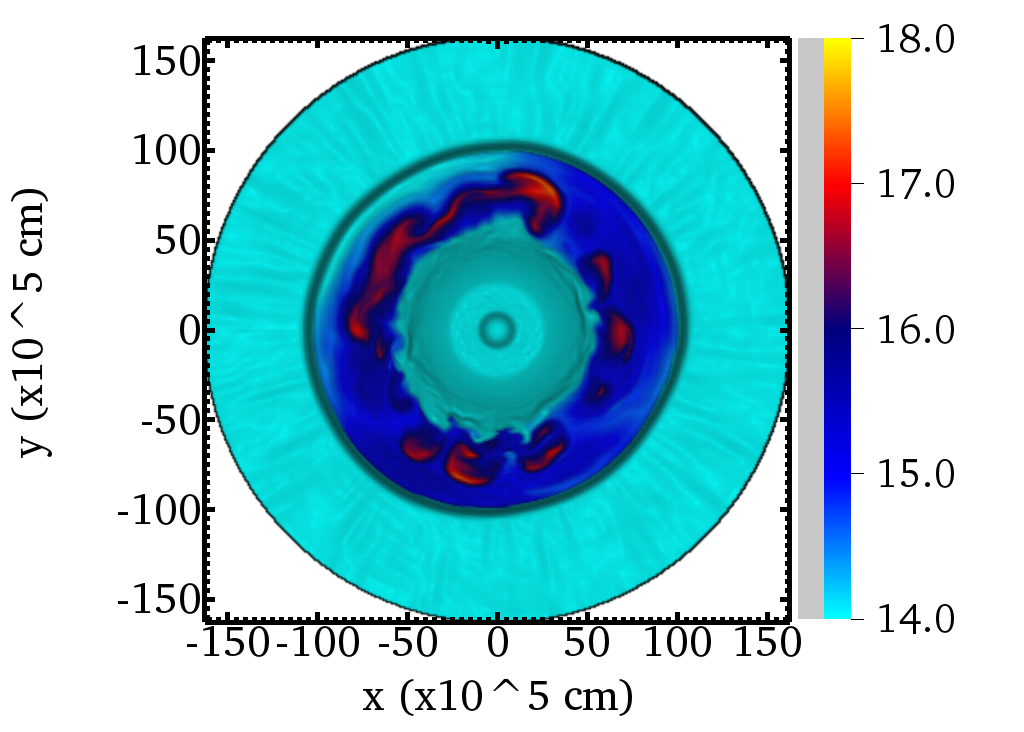
\includegraphics[width=0.49\textwidth]{./images/paper2/2.png} \\
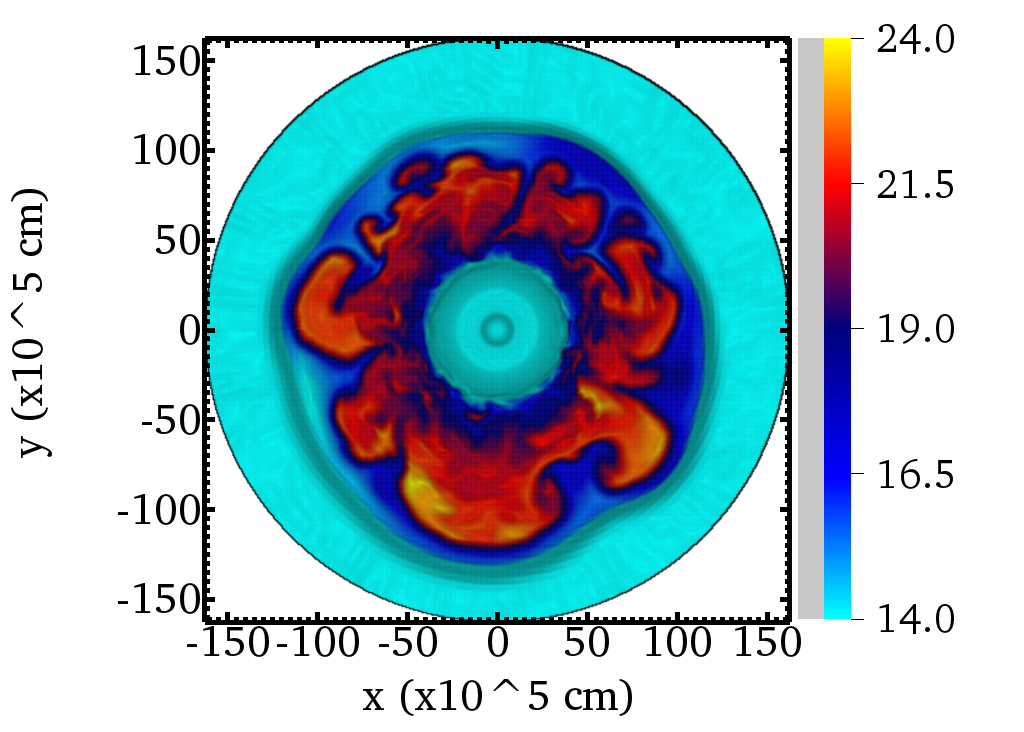
\includegraphics[width=0.49\textwidth]{./images/paper2/3.png}
\caption{The entropy per baryon in the xy-plane of the Yin-grid for model m15r. Shown at
at 167 (top left panel), 210 (top right panel), and 343 (bottom panel) ms post bounce. 
The entropy is given in units of Boltzmann's constant $k_b$. \label{figp2:sto}}
\end{figure}

The reduction of high-frequency GW emission generated by PNS convection can clearly be seen in model
m15r. Between $180$ and $250$ ms post bounce hot-bubble convection subsides and model m15r emits virtually no high-frequency GWs. The shock front reaches a minimum around $200$ ms post bounce, after
a $70$ ms long period of recession (\fig{figp2:rsh}). The small average shock radius favours SASI activity over
neutrino driven convection, and we see the development of low amplitude shock oscillations,
see the middle panel of \fig{figp2:sasi}. Convection, on the other hand, is quenched. 
\fig{figp2:sto} shows the entropy per baryon of model m15r, in the xy-plane of the Yin-grid.
The three panels show snapshots taken 167 (top left panel), 210 (top right panel), and 343 (bottom panel) ms
after core bounce. The top left and the bottom panel show the typical hot bubbles that are characteristic of
neutrino driven convection, but in the top right panel no such bubbles can be seen. 
The growth of low amplitude SASI activity and the suppression of convection in the post-shock layer is reflected
in the GW signal as weak emission at low frequencies and a complete absence of the high-frequency signal component.

\section{The standing accretion shock instability, rotation, and low-frequency gravitational wave emission}
There is no clear connection between development of SASI activity and the progenitor's initial rotation rate,
in the models we discuss in this chapter. Model m15r, in which the rotation profile is in accord with the stellar
evolution calculations, does not develop strong SASI activity. In both model m15nr and model m15fr, however, a strong spiral SASI mode emerges. 

Exactly how rotation influences the SASI growth rate and saturation is 
at the moment not clear. Recently \cite{blondin_17} studied the effects of rotation by means of idealised hydrodynamic simulations of a standing accretion shock (in 2D and 3D). The results of \cite{blondin_17} are in good agreement with the perturbative study of of \cite{yamasaki_08}, which found that the linear growth rate 
of non-axisymmetric SASI modes is an increasing function of the progenitor rotation rate.
However, in the non-linear regime \cite{kazeroni_17} does not find a monotonic connection between the
rotation and the saturation amplitude of the SASI. In fact Fig.3 of \cite{kazeroni_17} indicates that
SASI activity should decrease with increasing rotation rate, at low to moderate rotation rates. 

An additional complication comes from the fact that model m15nr was simulated with 
half the angular resolution of the other two models. Lower resolution has been found
to favour the growth SASI activity, because energy accumulates at larger scales \citep{hanke_12}.
However, \cite{abdikamalov_15} finds the opposite, and conclude that increasing the angular resolution 
reduces the SASI oscillations. They perform a set of general relativistic 3D hydrodynamic
simulations of a 27 \msun progenitor with a neutrino leakage scheme to study the phase between bounce and
shock revival.



